\justify
\fontsize{12pt}{14}\
\setlength{\parindent}{0cm}

\section{Actividad 3}
\normalsize El producto seleccionado para realizar los gráficos de oferta y demanda fue la yuca, esto se debe a que es uno de los productos más consumidos y producidos del departamento de Sucre la región en donde vivo. Así lo deja claro lo mencionado por \cite{hochschild2024} que menciona que solo en el munucipio de Corozal la yuca corresponde a tres cuartas partes de la producción total de estos tipos de cultivo. Así pues, tal cómo se evidencia en la figura \ref{fig:demanda} de la página \pageref{fig:demanda}, la demanda de este tubérculo varía de acuerdo al precio, de este modo a medida que el precio disminuye la demanda aumenta y viceversa. De igual modo, en la figura \ref{fig:oferta} de la página \pageref{fig:oferta} se observa que a medida que los precios aumentan la oferta aumenta y viceversa.

\begin{figure}[ht!]
    \centering
    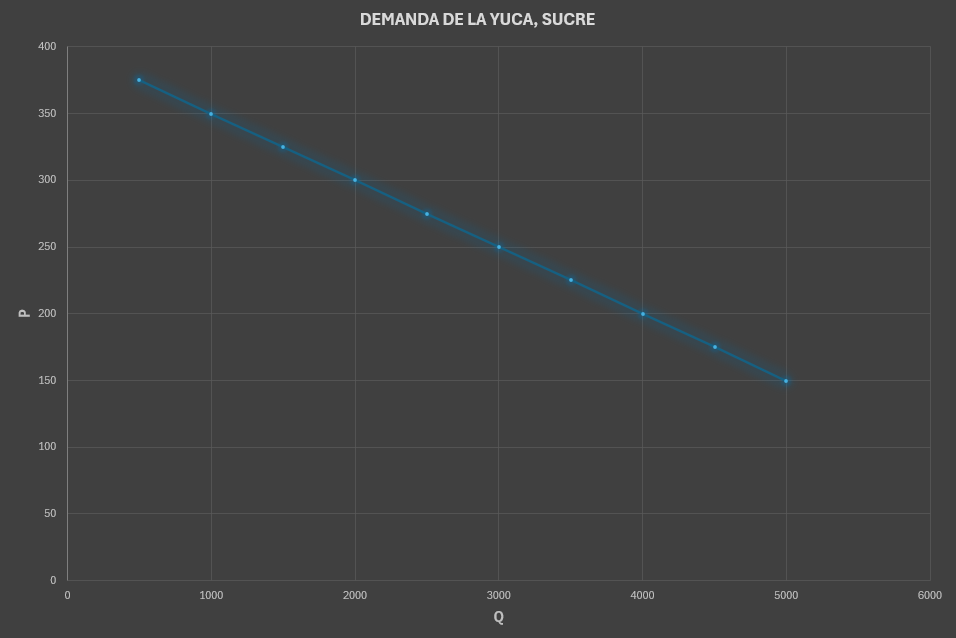
\includegraphics[width=15cm, height=13cm]{Demanda de la yuca}
    \caption{Diagrama de la demanda de la yuca en Sucre}
    \label{fig:demanda}
\end{figure}

\begin{figure}[ht!]
    \centering
    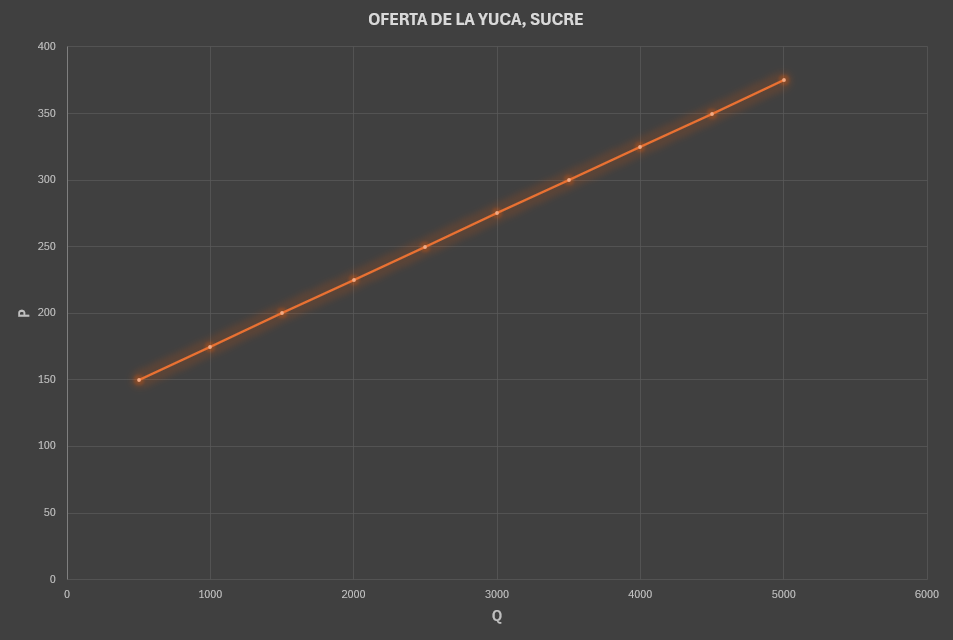
\includegraphics[width=15cm, height=13cm]{Oferta de la yuca}
    \caption{Diagrama de la oferta de la yuca en Sucre}
    \label{fig:oferta}
\end{figure}

\normalsize Teniendo en cuenta lo antes mencionado se puede evidenciar calaramente que entre más se abaraten los precios de la yuca, los consumidores demandan más el producto, esto influido, claro está, de la renta y expectativas de los clientes, así cómo tambien otras variables. De la misma manera, en el caso de la oferta, sucede lo contrario, entre más costoso sea el producto, los vendedores están más dispuestos a producir más, esto con la influencia de aspectos como los costos de producción y condiciones climáticas. Además de los antes mencionado, tal como se puede ver en la figura \ref{fig:equilibrio} de la página \pageref{fig:equilibrio}, el punto de equilibrio se encuentra con una oferta de 3000 tonelas a un precio de 275 pesos la unidad aproximadamente.

\begin{figure}[ht!]
    \centering
    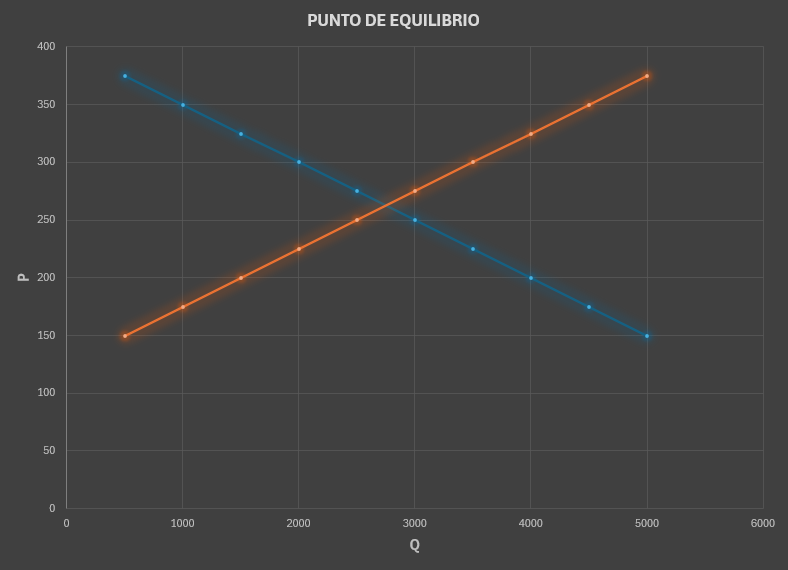
\includegraphics[width=15cm, height=13cm]{Punto de equilibrio}
    \caption{Diagrama del punto de equilibrio de la yuca en Sucre}
    \label{fig:equilibrio}
\end{figure}